
\section{Main simulation panel}
    This panel is the main part of the simulator user interface. Simulator simulates instruction set of PicoBlaze family and his copies.
    Following picture shows main window of the simulator. You can find here internal registers, scratchpad ram, input and output ports, stack,
    program counter, elapsed time and cycles, actual clock and internal flags: CARRY and ZERO. All those features can be edited during
    processor simulation. If some value changes state, it will turn yellow. You can drag out whole simulation panel and place it to, for example, another display.
    
   \begin{figure}[h!]
        \centering
        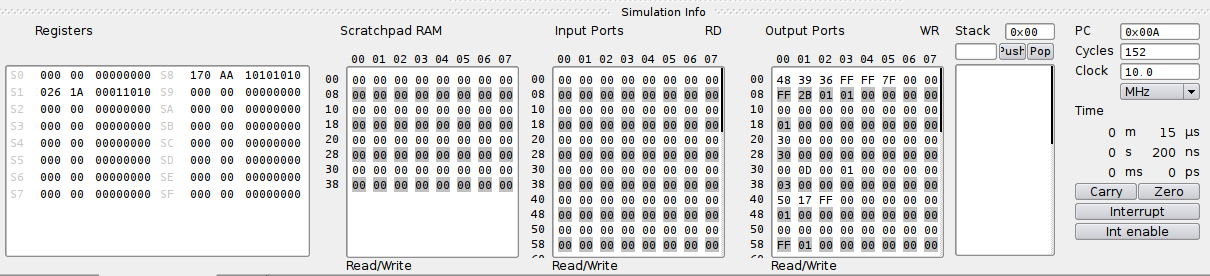
\includegraphics[width=\textwidth]{img/bottom_panel.png}
        \caption{Main simulator panel}
    \end{figure}

    \begin{description}
     \item [Register field] You can find here values of internal processor registers. First column represents name, second value in decimal, third
     hexadecimal and last binary.
     \item [Scratch-pad RAM] This hex editor represents values stored in scratch-pad RAM. Address of particular field is adition of line number
     and column number.
     \item [Ports] Output ports are represented by hex editors and you can determine value of each field by adition of column number and line number.
     You can also see status of picoblaze RD and WR pins. It can be usefull to see their status for better debuging.
     \item [Stack] Stack window represents actual values stored in stack. Top field represents virtual stack pointer and you can also push or pop values into the stack
     by inserting desired number to the field under "Stack" sign.
     \item [Info panel] Panel on the right side of simulation panel gives you general information about simulated code. You can find here program counter
     value, number of executed cycles, set  frekvency, elapsed time and Carry, Zero and Interrupt flag status. You can generate interrupt by clicking on "Interrupt button"
    \end{description}

    \subsection{Simulator warnings}
        MDS offers some warnings to ensure your debuging procces will be less painfull. It handles some common mistakes like PC overflow, stack overflow and
        some other problems. See pictures for more info or go to Interface -> Config -> Simulator warnings.
        
        \begin{table}[h!]
            \begin{tabular}{cc}
                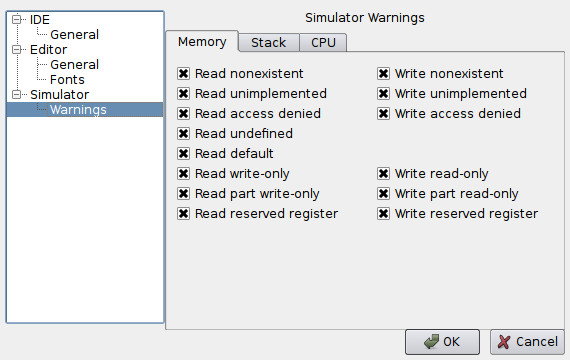
\includegraphics[width=.45\textwidth]{img/NewImg/interface4.png}
                    &
                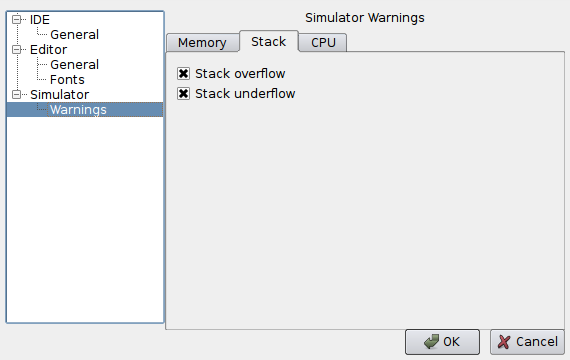
\includegraphics[width=.45\textwidth]{img/NewImg/interface5.png}
                    \\
                Simulator - Warnings -> Memory & Simulator - Warnings -> Stack
            \end{tabular}
        \end{table}

        \begin{table}[h!]
            \begin{tabular}{c}
                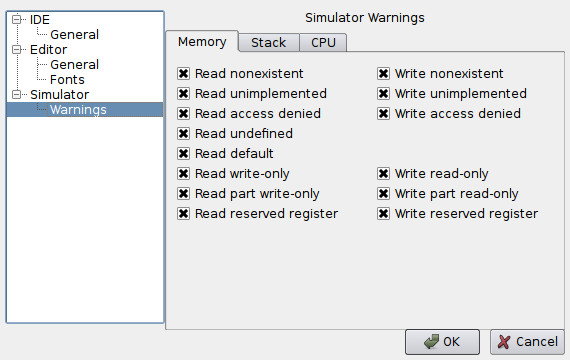
\includegraphics[width=.5\textwidth]{img/NewImg/interface4.png}
                \\
                Simulator - Warnings -> CPU 
            \end{tabular}
        \end{table}

    \subsection{Adding breakpoints and bookmarks}
        Our simulator supports breakpoints. The breakpoint is associated wth location in programming code that, when reached, triggers a temporary halt in the program.
        You can use breakpoints to test and debug programs by causing the program to stop at scheduled intervals so that the status of
        the program can be examined in stages. Note: Breakpoints will slow down the simulator. If you want maximum speed, click on top panel
        button dissable all breakpoints.
        
        Another usefull thing are bookmarks. When you are editiong one location in your source code multiple times, it is usefull to add a bookmark to it,
        so you can quickly get back when you need.
        
        \begin{figure}[h!]
            \centering
            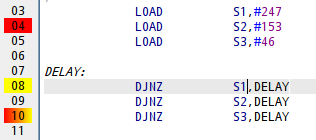
\includegraphics[width=.4\textwidth]{img/NewImg/breakpoints1.png}
            \caption{Yellow - bookmark, Red - breakpoint, Yellow/Red gradient - both}
        \end{figure}

    \subsection{Simulation cursor}
        Simulation cursor shows what instruction will be executed in next step. Two previous instructions are less and less highlighted, so you can track
        two previous steps. following figure displays actual cursor on line 8, one step before is on line 5 and another step is on 4.
        \begin{figure}[h!]
            \centering
            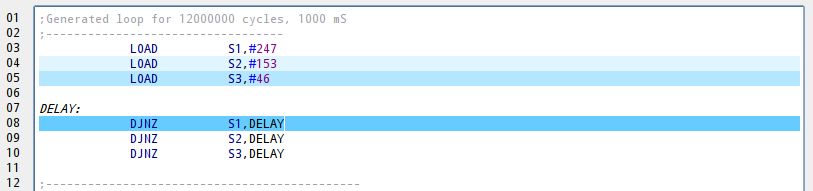
\includegraphics[width=\textwidth]{img/NewImg/simulationcursor1.png}
            \caption{Simulation cursor}
        \end{figure}
        
        MDS has special behavior when simulator encounters macro expansion. For better orientation, cursor will appear on two locations.
        On macro expansion and in macro declaration, showing your actual step. If you have macro expanded in your macro declaration, you will have
        three cursors and so on. For better understanding, following figure shows simulation cursor behavior with macros.
        \begin{figure}[h!]
            \centering
            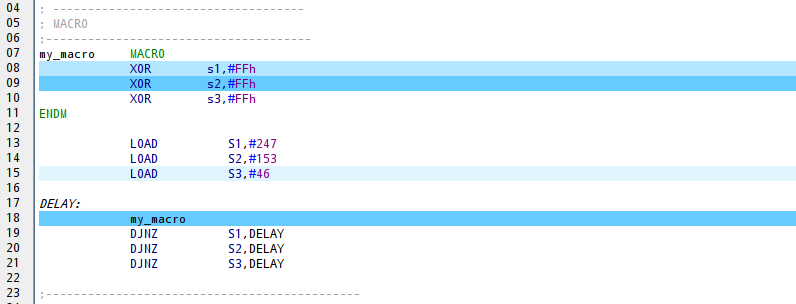
\includegraphics[width=\textwidth]{img/NewImg/simulationcursor2.png}
            \caption{Simulation cursor}
        \end{figure}        
    

    \subsection{List of macros, breakpoints and bookmarks}
        You can find important info about your simulation on the right panel. You can find here
    \begin{table}[h!]
        \begin{tabular}{ccc}
            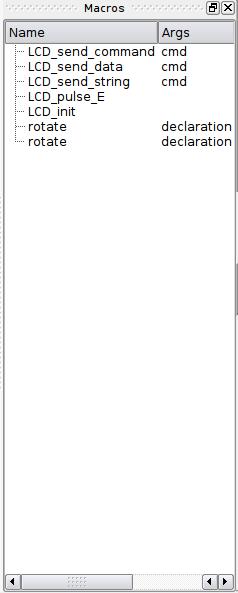
\includegraphics[width=.3\textwidth]{img/NewImg/listmacros.png}
                &
            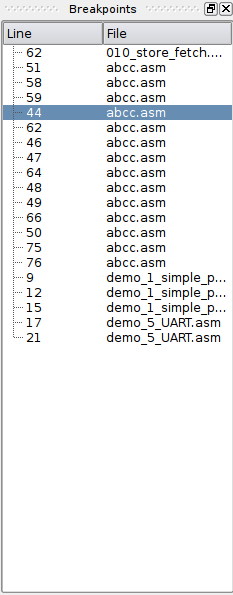
\includegraphics[width=.3\textwidth]{img/NewImg/listbreakpoints.png}
                &
            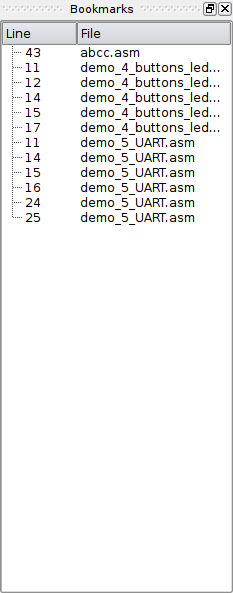
\includegraphics[width=.3\textwidth]{img/NewImg/listbookmarks.png}
            \\
            Macros & Breakpoints & Bookmarks
        \end{tabular}
    \end{table}

    
    \subsection{Modes of simulation}
        There are 4 modes of simulation:

        \begin{figure}[h!]
            \centering{}
            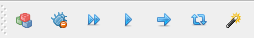
\includegraphics[width=.4\textwidth]{img/simulation_panel.png}
            \caption{Simulator toolbar.}
        \end{figure}

        \begin{itemize}
            \item STEP: Execute exactly one intruction, no matter how many machine cycles it will take. This does not apply for macro-instruction, in that case each instruction of the macro is executed separately.
            \item ANIMATE: Do the same as step, but in a loop, one after another until stopped by a waring condition or user request.
            \item RUN: This is generally the same as animate, but much faster, because GUI is not updated so often as in the animate mode.
            \item RESET: Resets everything to the initial state of program.
            \item UNHIGHLIGHT: Cleans up all highlighted text.

    %         \item STEP OVER: Execute as many instructions as possible until simulator cursor changes its location from one line of source code to another.
            \item ANIMATE: Do the same as step, but in a loop, one after another until stopped by a waring condition or user request.
            \item RUN: This is generally the same as animate, but much faster, because GUI is not updated so often as in the animate mode.
    %         \item STEP BACK: Take back the last performed step. There is limited number of step which can be taken back.
        \end{itemize}
